\documentclass[12pt,a4paper]{article}
\usepackage[polish]{babel}
\usepackage[T1]{fontenc}
\usepackage[utf8x]{inputenc}
\usepackage{hyperref}
\usepackage{url}
\usepackage[]{algorithm2e}
\usepackage{listings}
\usepackage{graphicx}
\usepackage{color}
\usepackage{listings}

\lstloadlanguages{% Check Dokumentation for further languages ...
	C,
	C++,
	csh,
	Java
}

\definecolor{red}{rgb}{0.6,0,0} % for strings
\definecolor{blue}{rgb}{0,0,0.6}
\definecolor{green}{rgb}{0,0.8,0}
\definecolor{cyan}{rgb}{0.0,0.6,0.6}

\lstset{
	language=csh,
	basicstyle=\footnotesize\ttfamily,
	numbers=left,
	numberstyle=\tiny,
	numbersep=5pt,
	tabsize=2,
	extendedchars=true,
	breaklines=true,
	frame=b,
	stringstyle=\color{blue}\ttfamily,
	showspaces=false,
	showtabs=false,
	xleftmargin=17pt,
	framexleftmargin=17pt,
	framexrightmargin=5pt,
	framexbottommargin=4pt,
	commentstyle=\color{green},
	morecomment=[l]{//}, %use comment-line-style!
	morecomment=[s]{/*}{*/}, %for multiline comments
	showstringspaces=false,
	morekeywords={ abstract, event, new, struct,
		as, explicit, null, switch,
		base, extern, object, this,
		bool, false, operator, throw,
		break, finally, out, true,
		byte, fixed, override, try,
		case, float, params, typeof,
		catch, for, private, uint,
		char, foreach, protected, ulong,
		checked, goto, public, unchecked,
		class, if, readonly, unsafe,
		const, implicit, ref, ushort,
		continue, in, return, using,
		decimal, int, sbyte, virtual,
		default, interface, sealed, volatile,
		delegate, internal, short, void,
		do, is, sizeof, while,
		double, lock, stackalloc,
		else, long, static,
		enum, namespace, string},
	keywordstyle=\color{cyan},
	identifierstyle=\color{red},
}
\usepackage{caption}
\DeclareCaptionFont{white}{\color{white}}
\DeclareCaptionFormat{listing}{\colorbox{blue}{\parbox{\textwidth}{\hspace{15pt}#1#2#3}}}
\captionsetup[lstlisting]{format=listing,labelfont=white,textfont=white, singlelinecheck=false, margin=0pt, font={bf,footnotesize}}


\addtolength{\hoffset}{-1.5cm}
\addtolength{\marginparwidth}{-1.5cm}
\addtolength{\textwidth}{3cm}
\addtolength{\voffset}{-1cm}
\addtolength{\textheight}{2.5cm}
\setlength{\topmargin}{0cm}
\setlength{\headheight}{0cm}

\begin{document}
	
	\title{Modelowanie i analiza systemów informatycznych (Informatyka st. II sem. 2)\\\small{Dokumentacja projektu nr 2}}
	\author{Dawid Bitner, Daniel Broczkowski, Damian Kwaśniok}
	\date{\today}

	\maketitle
	\newpage
	\section*{Część I}
	\subsection*{Opis programu}
	Zaprojektowano system wspomagania lekarza (poprzez użycie sieci neuronowej) poprzez automatyczną analizę danych medycznych. System posiada następujące funkcjonalności:
	
    a) ma dwa tryby -- uczenie algorytmu/klasyfikacja nowej próbki
    
    b) dane medyczne są szyfrowane i bezpieczne
    
    c) dane lekarzy są szyfrowane
    
    d) możliwość dodania nowego pacjenta/lekarza.
    
    Moduły zostały przetestowane, wykonano testy automatyczne i regresyjne. Sieć neuronowa została przeanalizowana pod względem ilości neuronów/warstw.
    
	\subsection*{Instrukcja obsługi}
    \subsubsection{Instalacja środowiska, wdrożenie projektu}
    Aby uruchomić backend należy:
    
    a) przejść do folderu ./src/
    
    b) wykonać kolejno polecenia: dotnet restore
    
    c) dotnet ef database update --project medic-decision-support-system
    
    d) uruchomienie testów: dotnet test
    
    e) dotnet run --project medic-decision-support-system
    
    
    
    Aby uruchomić część kliencką w trybie deweloperskim należy:
    
    a) w folderze z plikami frontendowymi wykonać polecenie npm install
    
    b) uruchomić serwer: ng serve --open
    
    Dzięki wbudowanym funkcjom .NET baza danych, w przypadku zainstalowanego systemu bazodanowego \textit{PostgreSQL}, odpowiednia baza wraz z tabelami, oraz domyślnymi użytkownikami automatycznie tworzy się w systemie.


	\subsection{Instrukcja wdrożenia}
W celu uruchomienia całego systemu aplikacji zawierającego część frontendową jak i backendową wymagane jest by na komputerze był zainstalowany system operacyjny pozwalający na instalację i kompilację programów .NET w wersji > 3.5 oraz Node.Js w wersji > 12.0.
W systemie powinny być zainstalowane właśnie te dwa środowiska.

	\subsection*{Podział prac}

Dawid Bitner - projekt bazy danych, dokumentacja, część frontendowa,\newline
Daniel Broczkowski - część frontendowa, dokumentacja,\newline
Damian Kwaśniok -  część backendowa, dokumentacja.

	\newpage
	\section*{Część II}
	\subsection*{Opis działania} 
Pacjenci po zalogowaniu posiadają możliwość przeglądania wyników badań należących do nich. Administrator może dodać dwa rodzaje użytkowników: Lekarz i Pacjent. Administrator, czy też lekarz ma możliwość wprowadzenia danych do systemu (ręcznie). Może również wykonać predykcję, sprawdzić za pomocą sieci neuronowej czy wyniki danego badania wskazują na istnienie cukrzycy u pacjenta, czy też nie. Posiada również możliwość przetrenowania modelu decyzyjnego.

	\subsection*{Diagram UML}
Medic API: \newline
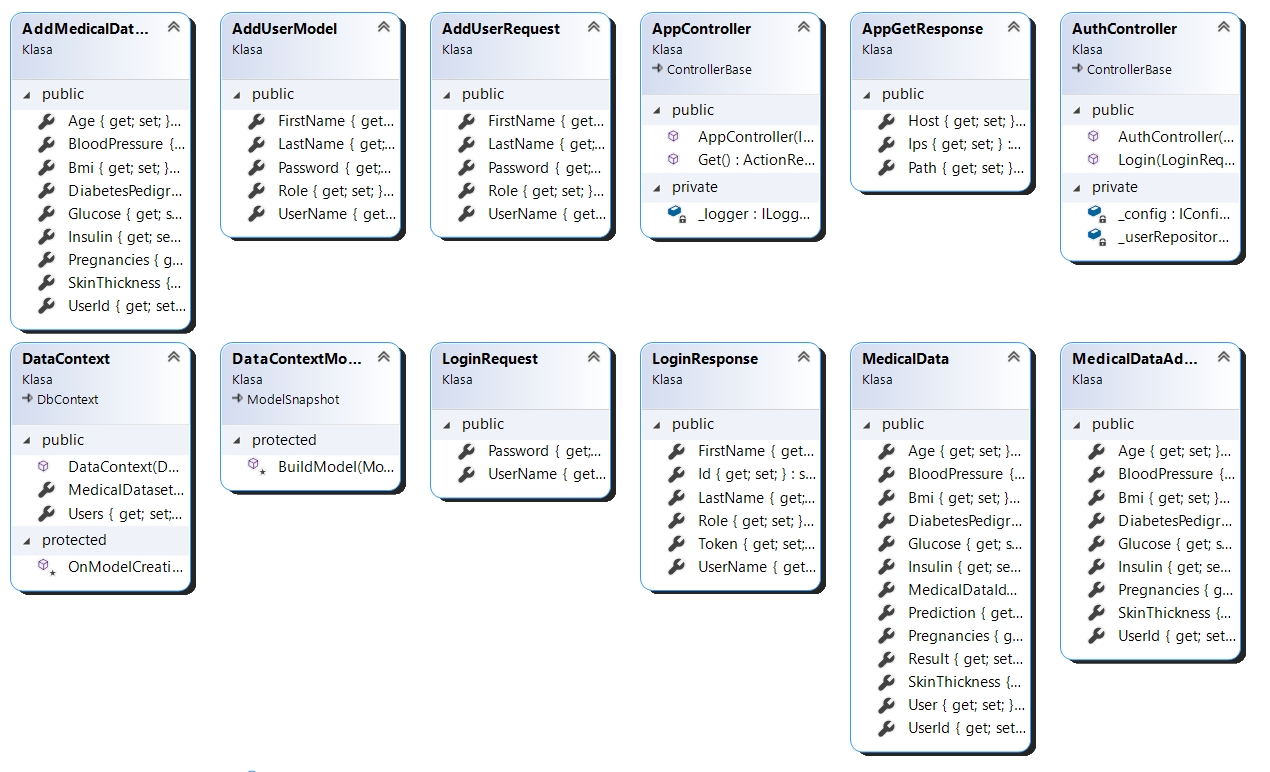
\includegraphics[scale=0.6]{diagram1.png} \newpage
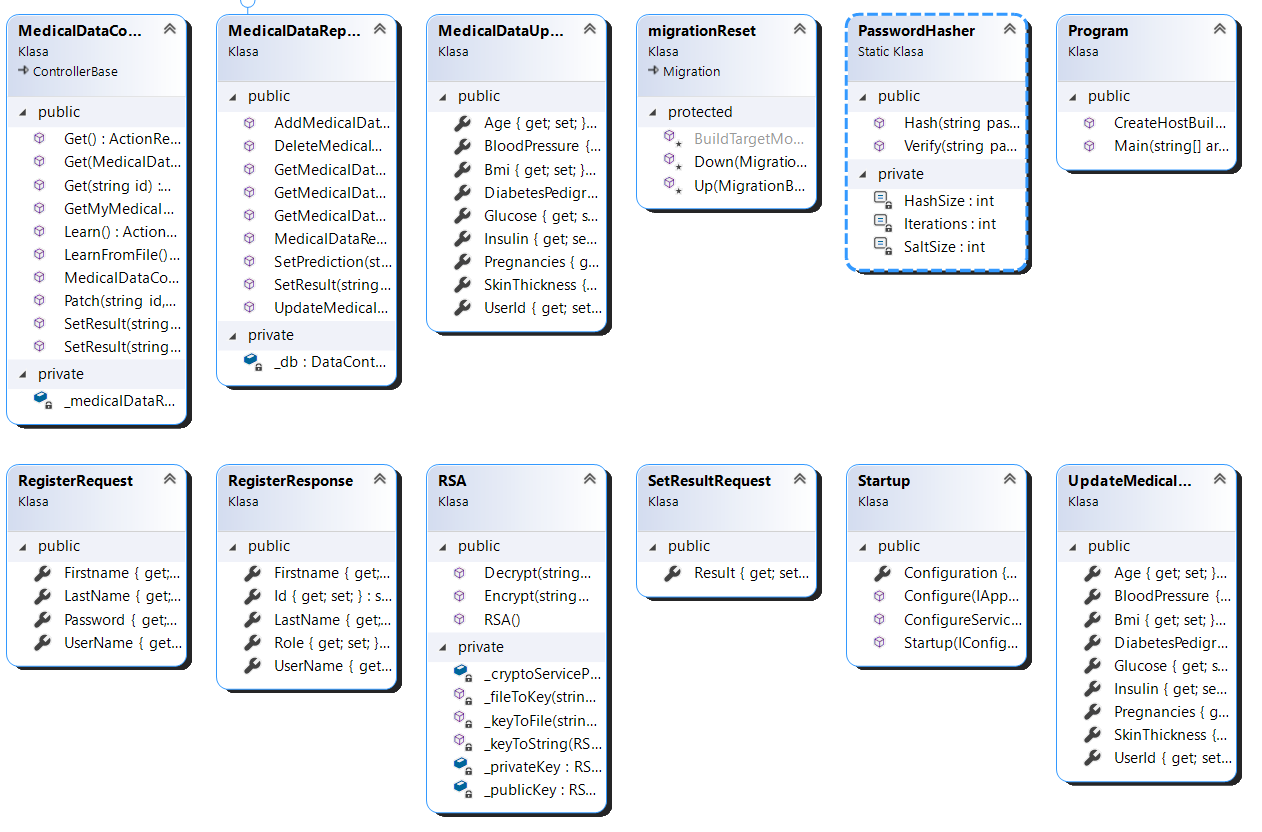
\includegraphics[scale=0.6]{diagram2.png} \newline
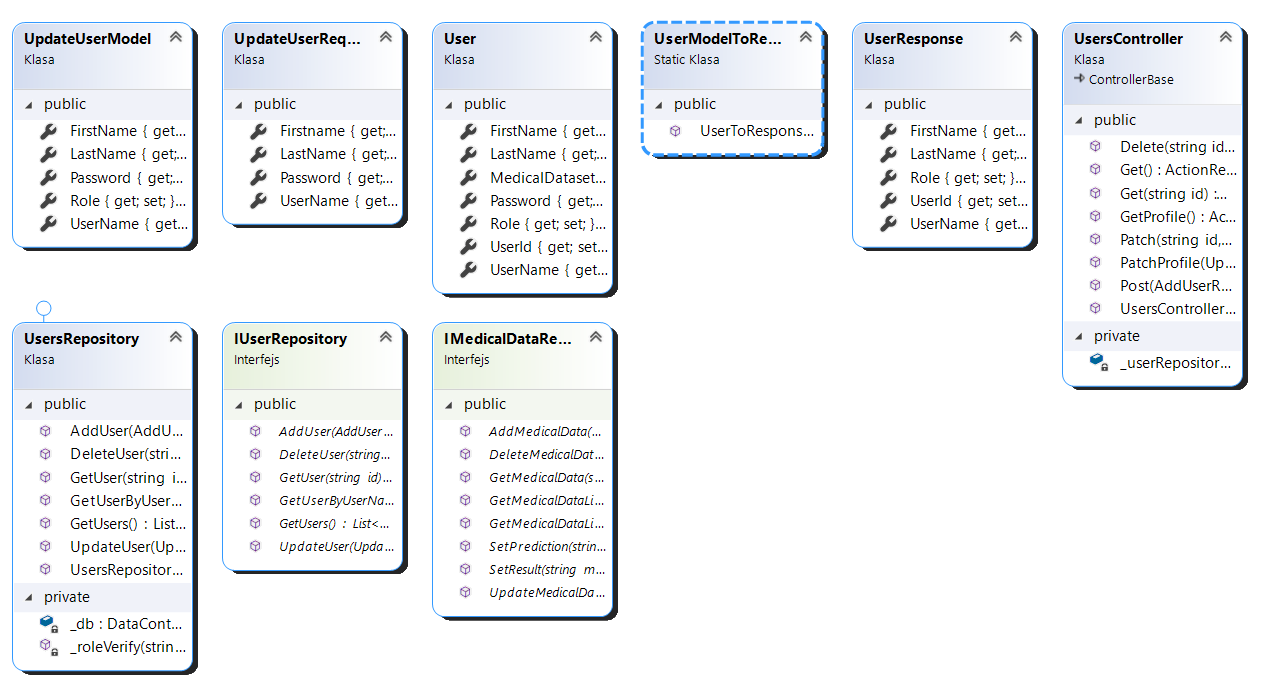
\includegraphics[scale=0.6]{diagram3.png} \newpage
Medic AI: \newline
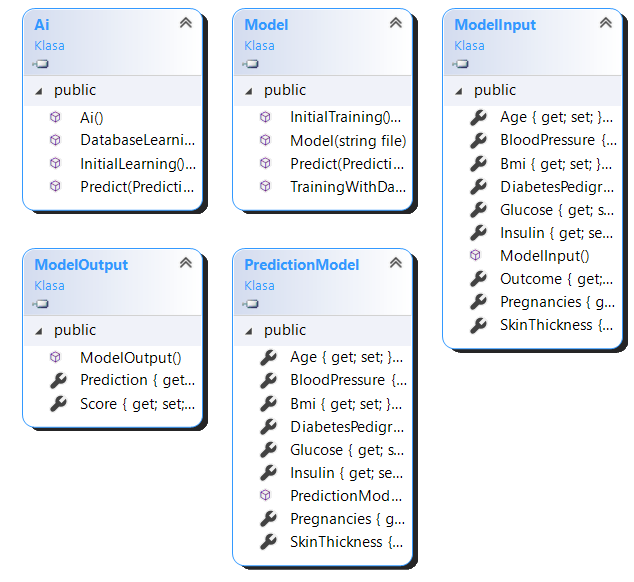
\includegraphics[scale=0.6]{diagram4.png}

 \subsection{Model sieci neuronowej}
	\begin{lstlisting}
	 private double Training(IDataView data, MLContext ctx)
        {
            var split = ctx.Data.TrainTestSplit(data, testFraction: 0.18);

            var features = split.TrainSet.Schema
                .Select(col => col.Name)
                .Where(col => col != "Label")
                .ToArray();
            var trainer =  new LbfgsLogisticRegressionBinaryTrainer.Options()
            {
                MaximumNumberOfIterations = 100,
            };
            var pipeline = ctx.Transforms.Concatenate("Features", features)
                .Append(ctx.BinaryClassification.Trainers.Gam(learningRate: 0.052, numberOfIterations: 25000));

            var model = pipeline.Fit(split.TrainSet);

            var predictions = model.Transform(split.TestSet);

            var metrics = ctx.BinaryClassification.Evaluate(predictions);

            ctx.Model.Save(model, data.Schema, "model.zip");
            _model = model;
            return metrics.Accuracy;
        }
	\end{lstlisting}
	\newpage
	\begin{lstlisting}
	public ModelOutput Predict(PredictionModel input)
        {
            var ctx = new MLContext();
            var model = ctx.Model.Load("model.zip", out _);
            PredictionEngine<ModelInput, ModelOutput> predictionEngine =
                ctx.Model.CreatePredictionEngine<ModelInput, ModelOutput>(model);
            ModelInput data = new ModelInput()
            {
                Age = input.Age,
                Bmi = input.Bmi,
                Glucose = input.Glucose,
                Insulin = input.Insulin,
                Pregnancies = input.Pregnancies,
                BloodPressure = input.BloodPressure,
                SkinThickness = input.SkinThickness,
                DiabetesPedigreeFunction = input.DiabetesPedigreeFunction,
            };
            ModelOutput prediction = predictionEngine.Predict(data);
            return prediction;
        }
	\end{lstlisting}
	 
	Model sieci neuronowej, który został użyty w aplikacji składa się z dwóch warstw. Sieć neuronowa jest oparta na klasyfikacji binarnej przy użyciu klasyfikatora opartego na binarnej regresji logistycznej o maksymalnej ilości 100 iteracji. Ze względu na specyfikę problemu, chcąc otrzymać wynik przewidywania, czy pacjent jest zdrowy lub chory została użyta klasyfikacja binarna. Jako wartość tempa uczenia sieci neuronowej (learningRate) została przyjęta wartość 0.052, natomiast za łączną liczbę przebiegów danych treningowych przyjęto liczbę 25000. Dane treningowe stanowiły 18\% zbioru danych.
    
    \subsection*{Opis komponentów systemu}
    
    \subsubsection*{Panel rejestracji}
    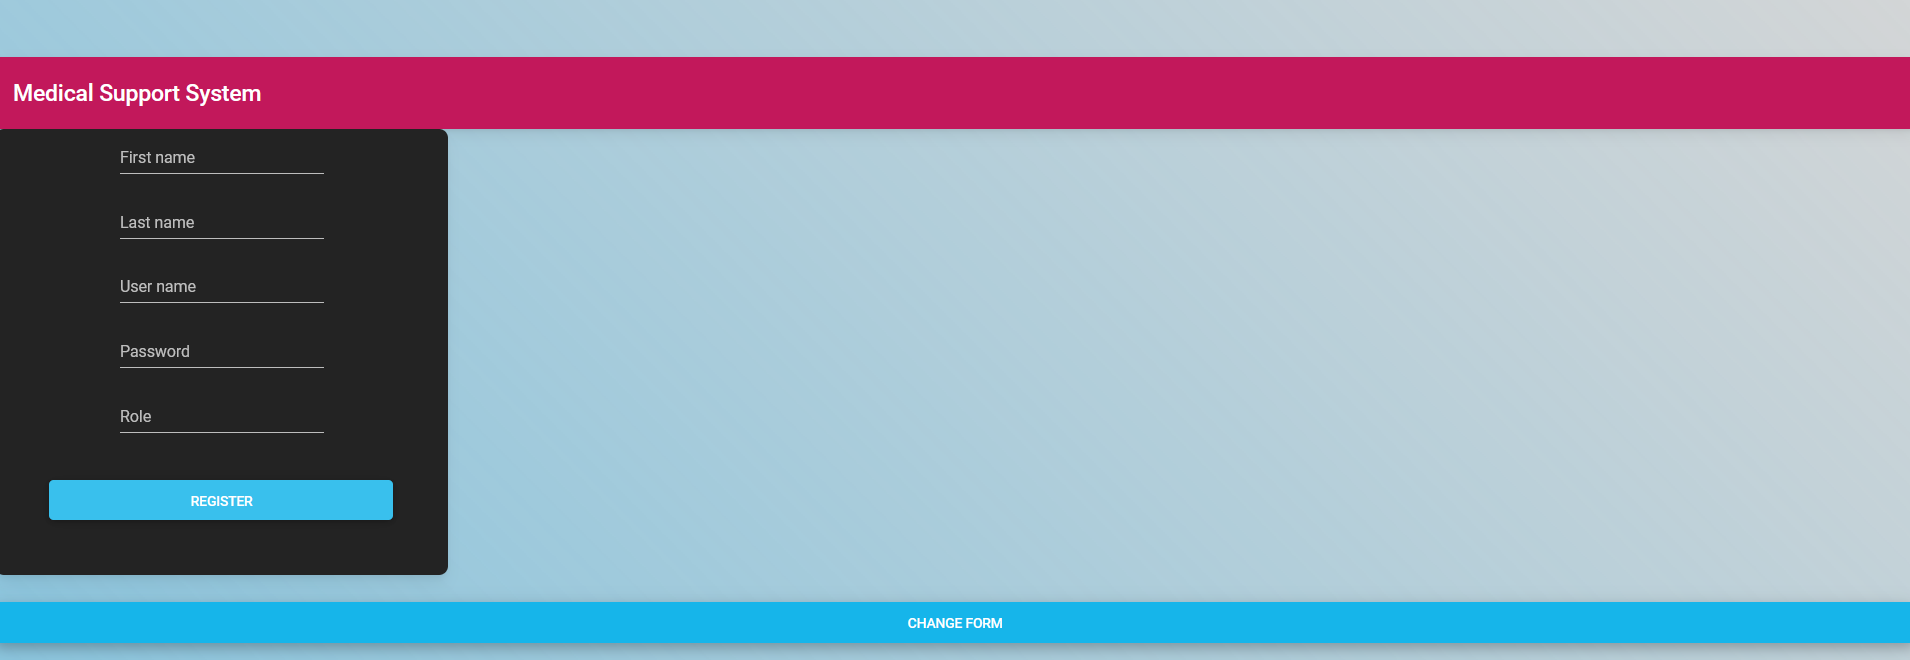
\includegraphics[width=\textwidth,height=\textheight,keepaspectratio]{register.png}
    Do rejestracji wymagane jest podanie imienia, nazwiska, loginu oraz hasła i typu konta.
    
    \subsubsection*{Panel logowania}
    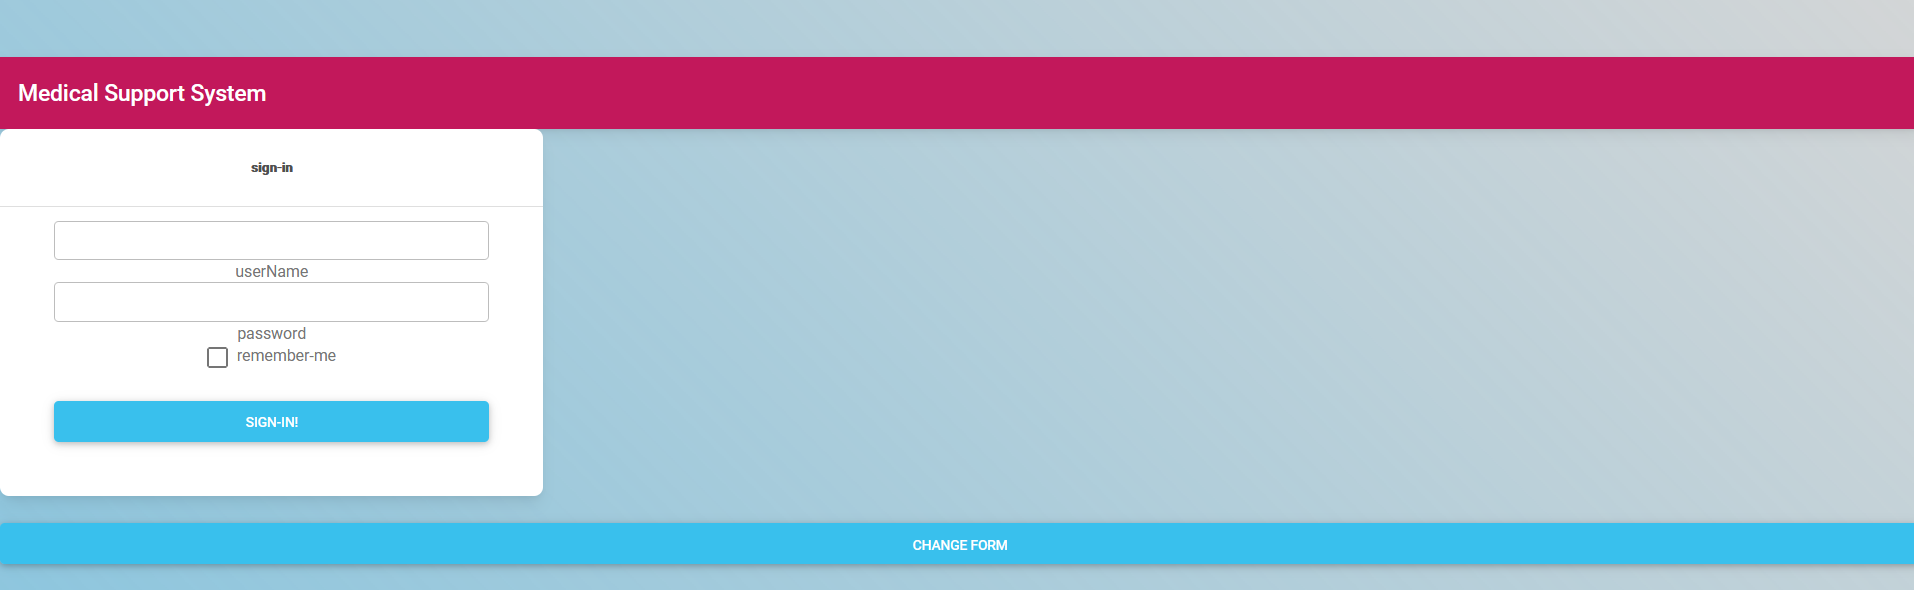
\includegraphics[width=\textwidth,height=\textheight,keepaspectratio]{login.png}
    W celu zalogowania należy wprowadzić właściwe dane logowania.
    
    \subsubsection*{Panel dodawania danych medycznych}
    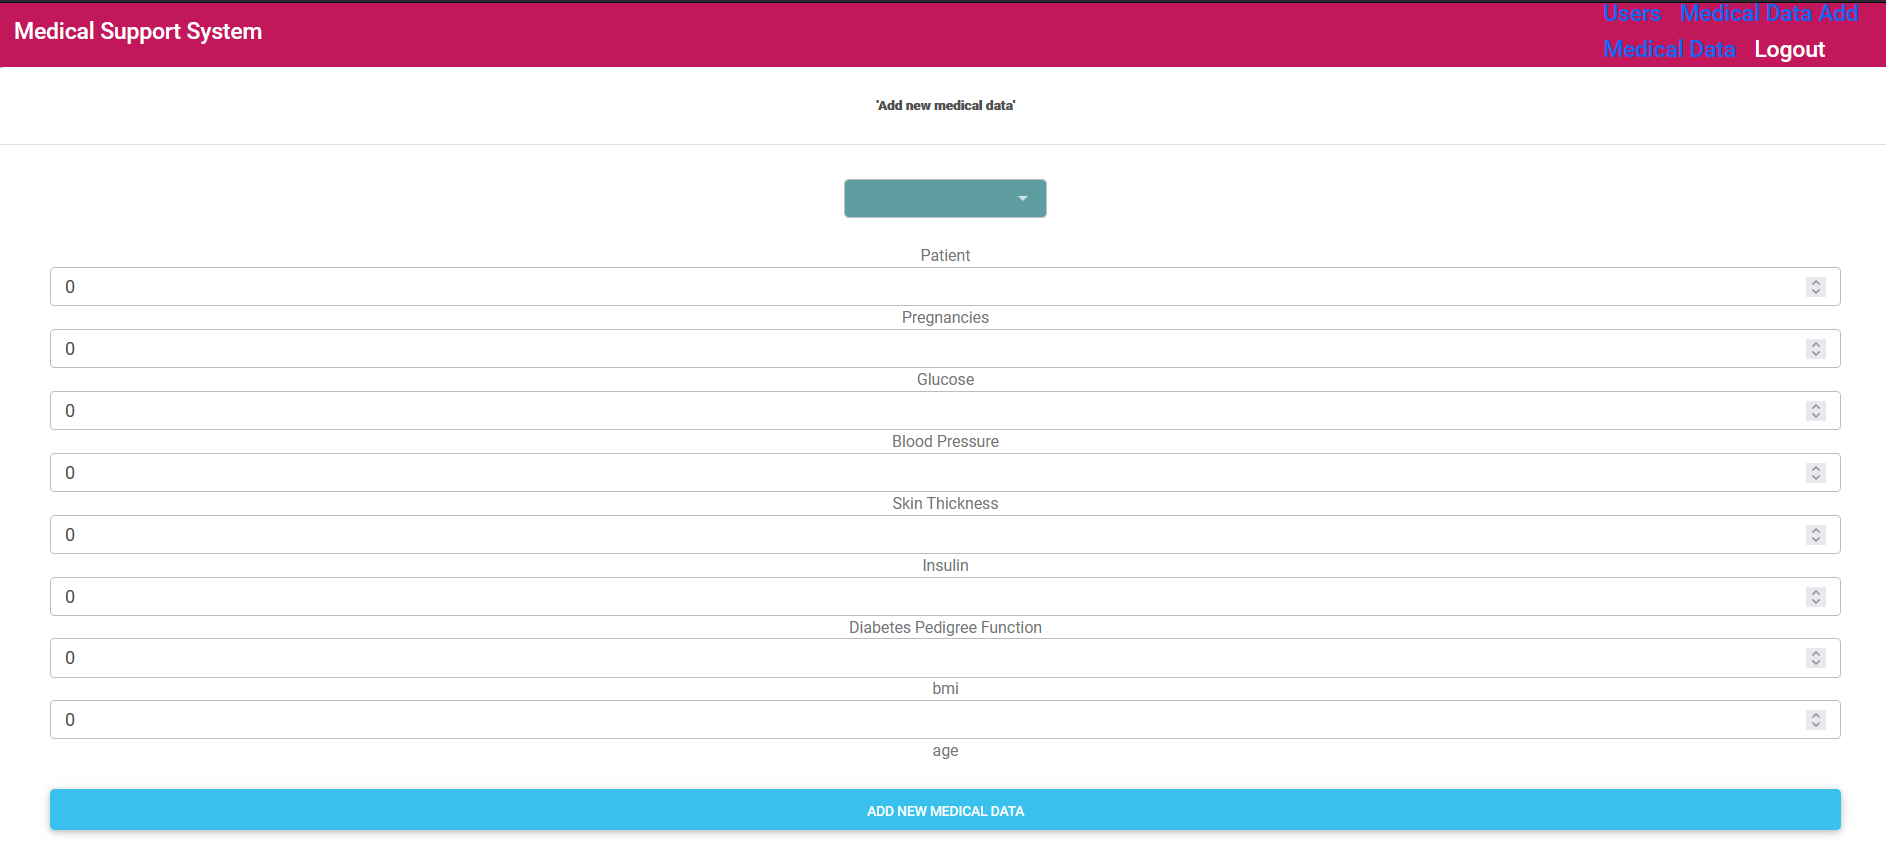
\includegraphics[width=\textwidth,height=\textheight,keepaspectratio]{Add_medical_data.png}
    \newline
    Należy wybrać pacjenta z listy oraz uzupełnić dane reprezentujące jego dane medyczne.
    
    \subsubsection*{Panel widoku danych medycznych}
    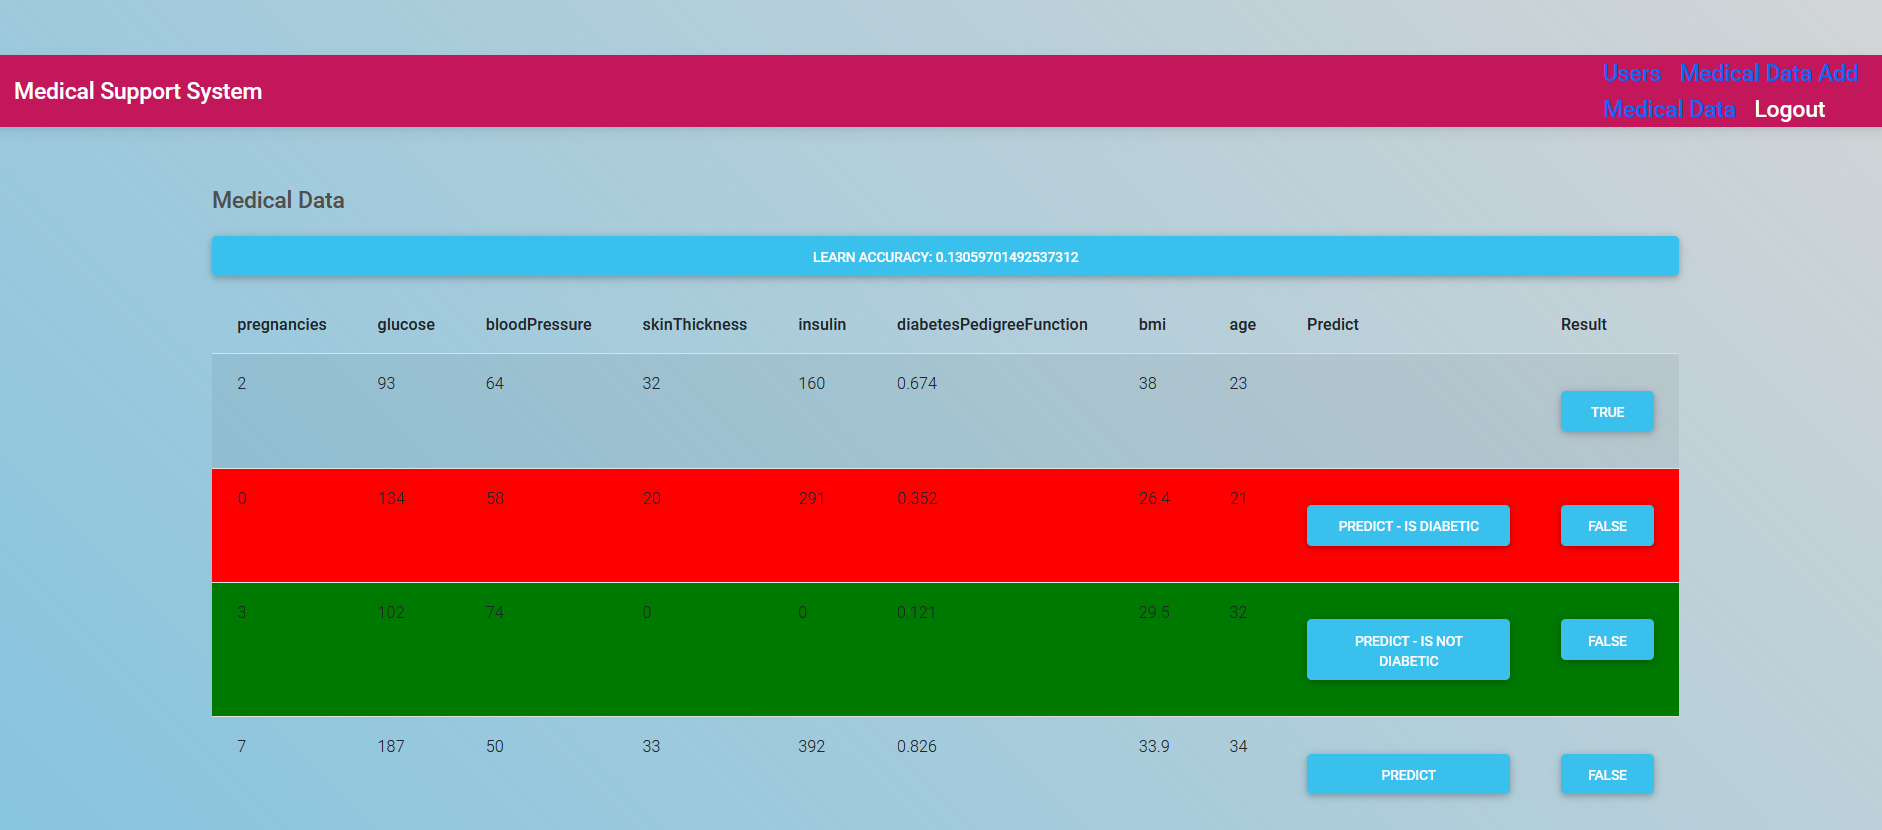
\includegraphics[width=\textwidth,height=\textheight,keepaspectratio]{view_medical_data.png}
    \newline
    Panel ten składa się z kilku części i funkcjonalności. \newline
    Na górze panelu znajduje się przycisk \textbf{Learn}. Po kliknięciu tego przycisku zostanie uruchomione uczenie sieci, a następnie wynik tego uczenie zostanie dopisany w treści przycisku.\newline
    Główną cześć widoku stanowi tabela wyświetlająca dane medyczne wprowadzone do systemu. Każdy wiersz posiada dodatkowo dwie kolumny z akcjami do wykonania:\newline
    \textbf{Predict} - służy to klasyfikacji próbki. Klasyfikacja może zostać uruchomiona tylko dla próbek nieoznaczonych jako \textit{TRUE} (nieprzeznaczonych do uczenia sieci) albo świeżych próbek wprowadzonych do systemu. Po dokonaniu klasyfikacji w przycisku zostanie zaprezentowany rezultat klasyfikacji oraz dodatkowo wiersz zostanie odpowiednio pokolorowany\newline
    \textbf{Result} - służy do oznaczania próbki jako próbki, która ma zostać użyta do uczenia sieci.
    \newline \newline
    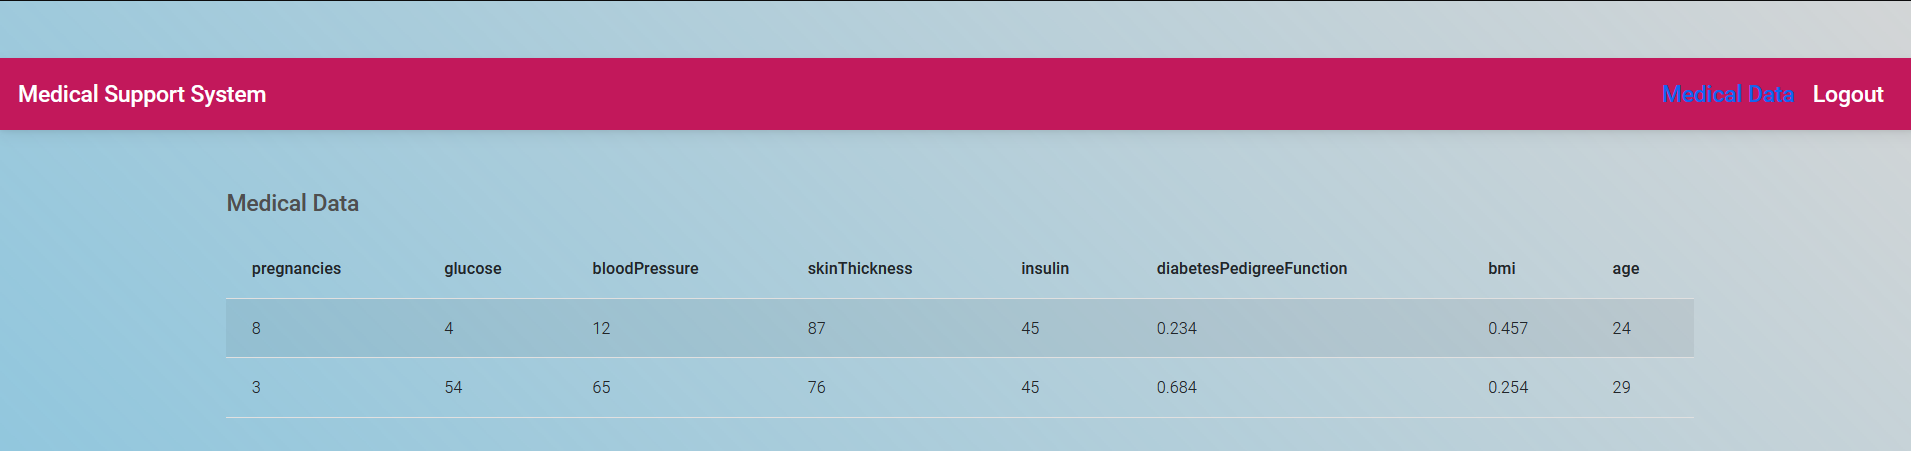
\includegraphics[width=\textwidth,height=\textheight,keepaspectratio]{view_medical_data_patient.png} \newline
    Widok pacjenta ogranicza się do widoczności próbek, które należą tylko do niego. Nie może uruchomić uczenia sieci oraz klasyfikacji próbek,
    

	\subsection*{Algorytm szyfrowania}
Algorytm RSA składa się z trzech podstawowych kroków:

    a) Generacja klucza publicznego i tajnego. Klucz publiczny jest przekazywany wszystkim zainteresowanym i umożliwia zaszyfrowanie danych. Klucz tajny umożliwia rozszyfrowanie danych zakodowanych kluczem publicznym. Jest trzymany w ścisłej tajemnicy.

    b) Użytkownik po otrzymaniu klucza publicznego, np. poprzez sieć Internet, koduje za jego pomocą swoje dane i przesyła je w postaci szyfru RSA do adresata dysponującego kluczem tajnym, np. do banku, firmy komercyjnej, tajnych służb. Klucz publiczny nie musi być chroniony, ponieważ nie umożliwia on rozszyfrowania informacji - proces szyfrowania nie jest odwracalny przy pomocy tego klucza. Zatem nie ma potrzeby jego ochrony i może on być powierzany wszystkim zainteresowanym bez ryzyka złamania kodu.

    c) Adresat po otrzymaniu zaszyfrowanej wiadomości rozszyfrowuje ją za pomocą klucza tajnego.
    \newline\newline
    Zalety: \newline
    - Algorytm RSA jest bezpieczny dla swoich użytkowników dzięki zastosowaniu złożonych algorytmów matematycznych. \newline
    - Algorytm RSA jest trudny do złamania, ponieważ obejmuje faktoryzację liczb pierwszych, które są trudne do faktoryzacji. \newline
    \newline
    Wady:\newline
    -Algorytm RSA może działać bardzo wolno w przypadkach, gdy duże dane muszą być szyfrowane przez ten sam komputer. \newline
    -Wymaga weryfikacji wiarygodności kluczy publicznych przez stronę trzecią. 
    -Dane przesyłane za pomocą algorytmu RSA mogą zostać naruszone przez pośredników w trakcie wymiany danych, którzy mogą spreparować system klucza publicznego, tak by był przez nich znany. \newline
    \newline
    Pomimo wad, RSA jest uważany obecnie za jeden z najbezpieczniejszych sposobów szyfrowania danych.
    
    Implementacja:
\begin{lstlisting}
using System;
using System.IO;
using System.Security.Cryptography;
using System.Text;
using System.Xml;
using System.Xml.Serialization;

namespace medic_api.Helpers
{
    public class RSA
    {
        private static RSACryptoServiceProvider _cryptoServiceProvider = new RSACryptoServiceProvider(2048);
        private readonly RSAParameters _privateKey;
        private readonly RSAParameters _publicKey;

        public RSA()
        {
            _privateKey = _fileToKey("privateKey.xml");
            _publicKey = _fileToKey("publicKey.xml");
        }

        private RSAParameters _fileToKey(string filename)
        {
            try
            {
                XmlDocument xmlDocument = new XmlDocument();
                xmlDocument.Load(filename);
                XmlSerializer xmlSerializer = new XmlSerializer(typeof(RSAParameters));
                XmlReader xmlReader = new XmlNodeReader(xmlDocument.DocumentElement);
                var key = (RSAParameters) xmlSerializer.Deserialize(xmlReader);
                return key;
            }
            catch
            {
                var key =_cryptoServiceProvider.ExportParameters(true);
                _keyToFile(_keyToString(key), filename);
                return key;
            }
        }

        private void _keyToFile(string key, string filename)
        {
            XmlDocument xmlDocument = new XmlDocument();
            xmlDocument.LoadXml(key);
            xmlDocument.Save(filename);
        }

        private string _keyToString(RSAParameters key)
        {
            var stringWriter = new StringWriter();
            var xmlSerializer = new XmlSerializer(typeof(RSAParameters));
            xmlSerializer.Serialize(stringWriter, key);
            return stringWriter.ToString();
        }

        public string Encrypt(string plainText)
        {
            _cryptoServiceProvider = new RSACryptoServiceProvider();
            _cryptoServiceProvider.ImportParameters(_publicKey);
            var data = Encoding.UTF8.GetBytes(plainText);
            var cypher = _cryptoServiceProvider.Encrypt(data, true);
            return Convert.ToBase64String(cypher);
        }

        public string Decrypt(string cypher)
        {
            var dataBytes = Convert.FromBase64String(cypher);
            _cryptoServiceProvider.ImportParameters(_privateKey);
            var plainText = _cryptoServiceProvider.Decrypt(dataBytes, true);
            return Encoding.UTF8.GetString(plainText);
        }
    }
}
\end{lstlisting}	

    \newpage
	\subsection*{Bazy danych}
Struktura bazy danych projektu prezentuje się następująco:
\begin{figure}[h!]
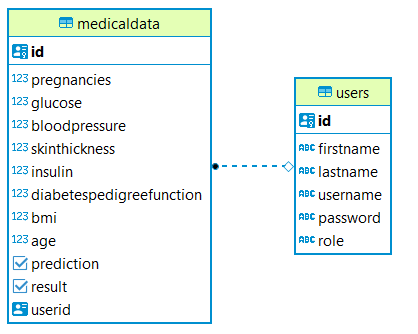
\includegraphics{img/baza.png}
\end{figure}  

Baza danych w projekcie została ograniczona do minimum. Stworzona jest w Postgresie. Posiada dwie tabele. Z badaniami i użytkownikami. Tabela badań zawiera parametry badań, oraz kolumnę z identyfikatorem użytkownika do którego należą badania. Natomiast tabela użytkowników zawiera informacje o nich, w tym przypisaną rolę w systemie.

	\subsection*{Zalety i wady systemów eksperckich}
System ekspertowy to system komputerowy zawierający w sobie wyspecjalizowaną  wiedzę  na  temat  określonego obszaru  ludzkiej  działalności,  przy  czym  wiedza ta jest tak zorganizowana, że umożliwia systemowi wejście w interakcyjny dialog z użytkownikiem,  w  wyniku  czego  system  może oferować rady lub podpowiadać decyzje, jak również objaśniać proces prowadzonego wnioskowania. System ekspercki może służyć m.in.: do diagnozowania chorób, a raczej dopomocy przy ich diagnozowaniu, jak na przykład ma to miejsce w tym projekcie.
\newline\newline
Do głównych zalet systemów eksperckich można zaliczyć:\newline
- mniejszy koszt pojedynczej ekspertyzy\newline
- automatyczne wyjaśnianie decyzji\newline
- szybkość uzyskania ekspertyzy\newline
- stała, niewrażliwa na emocje i czynniki zewnętrzne ekspertyza\newline
- uczenie metodą prób i błędów\newline
- inteligentny interfejs człowiek-komputer\newline
\newline\newline
Naszym zdaniem do głównych wad systemów eksperckich należą m.in.:\newline
- Konieczność wykonania treningu na najlepiej dużym zbiorze danych, gdzie możemy nie mieć pewności że rezultaty są poprawne\newline
- Wiedza przetwarzana jest w sposób mechaniczny\newline
- Wąski zakres\newline
- Zasugerowany wynik przez system może wpływać na decyzję człowieka w przypadku gdy użytkownik systemu zbyt mocno ufa wynikowi podanemu przez system.\newline

	\subsection*{Implementacja systemu eksperckiego}
	\begin{lstlisting}
        public ActionResult<double> Learn()
        {
            Ai ai = new Ai();
            var data = _medicalDataRepository.GetMedicalDataList().Where(d => d.Result != null).ToList();
            var preparedList = new List<ModelInput>();
            foreach (var medicalData in data)
            {
                var item = new ModelInput()
                {
                    Age = medicalData.Age,
                    Bmi = (float)medicalData.Bmi,
                    Glucose = medicalData.Glucose,
                    Insulin = medicalData.Insulin,
                    Outcome = medicalData.Result != null && (bool) medicalData.Result,
                    Pregnancies = medicalData.Pregnancies,
                    BloodPressure = medicalData.BloodPressure,
                    SkinThickness = medicalData.SkinThickness,
                    DiabetesPedigreeFunction = (float) medicalData.DiabetesPedigreeFunction,
                };
                preparedList.Add(item);
            }

            if (preparedList.Count < 15)
            {
                return Problem("Not enough data");
            }
            var accuracy = ai.DatabaseLearning(preparedList);
            return Ok(accuracy);
        }
        
        public ActionResult<string> SetResult(string id, [FromBody] SetResultRequest body)
        {
            var resultId = _medicalDataRepository.SetResult(id, body.Result);
            return Ok(resultId);
        }
	\end{lstlisting}
	
	\subsection*{Testy}
Wszystkie testy w aplikacji na ten moment kończą się sukcesem:
\begin{figure}[h!]
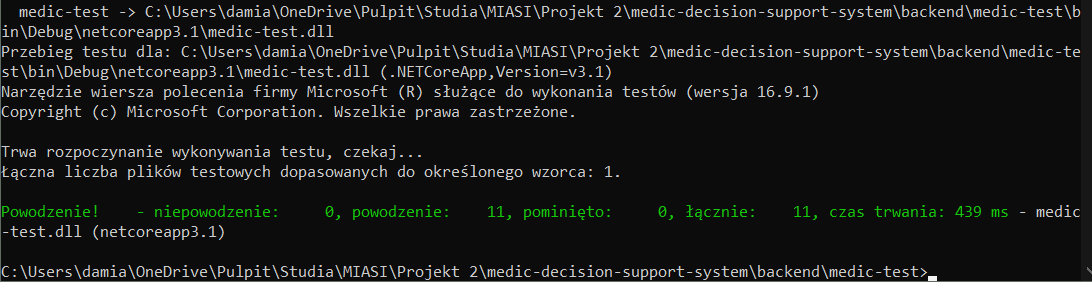
\includegraphics[scale=0.65]{testy.png}
\end{figure}
	
Zostały przeprowadzone następujące kilka testów dotyczących pobierania danych medycznych:
	\begin{lstlisting}
using System;
using System.Collections.Generic;
using System.Net.Http;
using System.Security.Claims;
using System.Security.Principal;
using medic_api.Controllers.MedicalData;
using medic_api.DAL.Models;
using medic_api.DAL.Repository.MedicalData;
using Microsoft.AspNetCore.Http;
using Microsoft.AspNetCore.Mvc;
using Moq;
using Xunit;

namespace medic_test.Controllers
{
    public class MedicalDataControllerTest
    {
        [Fact]
        public void MedicalDataControllerGet()
        {
            var newId = new Guid();
            var mock = new Mock<IMedicalDataRepository>();
            var controller = new MedicalDataController(mock.Object);
            var data = controller.Get(newId.ToString());
            mock.Verify(x => x.GetMedicalData(newId.ToString()), Times.Once);
            Assert.IsType<ActionResult<MedicalData>>(data);
        }
        
        [Fact]
        public void MedicalDataControllerGetList()
        {
            var mock = new Mock<IMedicalDataRepository>();
            var controller = new MedicalDataController(mock.Object);
            var data = controller.Get();
            mock.Verify(x => x.GetMedicalDataList(), Times.Once);
            Assert.IsType<ActionResult<List<MedicalData>>>(data);
        }
        
        [Fact]
        public void MedicalDataControllerGetListByUser()
        {
            var newId = new Guid();
            var mock = new Mock<IMedicalDataRepository>();
            var user = new ClaimsPrincipal(new ClaimsIdentity(new Claim[]
            {
                new Claim(ClaimTypes.Sid, newId.ToString()),
            }, "mock"));
            
            var controller = new MedicalDataController(mock.Object);
            controller.ControllerContext = new ControllerContext()
            {
                HttpContext = new DefaultHttpContext() { User = user }
            };
            var data = controller.GetMyMedicalData();
            mock.Verify(x => x.GetMedicalDataListByUser(newId.ToString()), Times.Once);
            Assert.IsType<ActionResult<List<MedicalData>>>(data);
        }
    }
}
	\end{lstlisting}
	
	Przy pomocy biblioteki Xunit zostały przeprowadzone testy szyfrowania algorytmem RSA.
	\begin{lstlisting}
using System;
using medic_api.Helpers;
using Xunit;
using Xunit.Abstractions;

namespace medic_test
{
    public class Encryptor
    {
        [Fact]
        public void Encrypt()
        {
            RSA rsa = new RSA();
            RSA rsa2 = new RSA();
            string testCase = "Admin123 jakis test /n\n";
            var encrypted= rsa.Encrypt(testCase);
            var decrypted = rsa2.Decrypt(encrypted);
            Assert.Equal(testCase, decrypted);
        }
    }
}
	\end{lstlisting}
	
		\begin{lstlisting}
using medic_api.Helpers;
using Xunit;

namespace medic_test
{
    public class Hasher
    {
        [Theory]
        [InlineData("", "")]
        public void HasherTest(string expected, string input)
        {
            Assert.Equal(expected, PasswordHasher.Hash(input));
        }

        [Theory]
        [InlineData("some test", "some test", true)]
        [InlineData("some test", "some test 2", false)]
        [InlineData("some test 2", "some test", false)]
        [InlineData("", "", false)]
        [InlineData("a", "", false)]
        [InlineData("", "a", false)]
        public void Verify(string str, string str2, bool equal)
        {
            var hash = PasswordHasher.Hash(str);
            Assert.Equal(equal, PasswordHasher.Verify(str2, hash));
        }
    }
}
	\end{lstlisting}
	
	Pod koniec pisania projektu, pokrycie kodu testami wynosiło ok. 2 procent.
	
	\newpage
	\section*{Pełen kod programu}
	\subsubsection{AppGetResponse.cs}
	\begin{lstlisting}
using System.Collections.Generic;

namespace medic_api.Controllers.DTO
{
    public class AppGetResponse
    {
        public string Host { get; set; }
        public string Path { get; set; }
        public IList<string> Ips { get; set; }
    }
}
	\end{lstlisting}
	\subsubsection{AppController.cs}
	\begin{lstlisting}
using System;
using System.Collections.Generic;
using Microsoft.AspNetCore.Mvc;
using Microsoft.Extensions.Logging;
using System.Net;
using medic_api.Controllers.DTO;
using Microsoft.AspNetCore.Authorization;

namespace medic_api.Controllers
{
    [ApiController]
    [Route("api/[controller]")]
    [Authorize(Policy = "Patient")]
    public class AppController : ControllerBase
    {
        private readonly ILogger<AppController> _logger;

        public AppController(ILogger<AppController> logger)
        {
            _logger = logger;
        }

        [HttpGet]
        public ActionResult<AppGetResponse> Get()
        {
            IPAddress[] localIPs = Dns.GetHostAddresses(Dns.GetHostName());
            List<string> ipList = new List<string>();
            foreach (var ipAddress in localIPs)
            {
                ipList.Add(ipAddress.ToString());
            }

            AppGetResponse response = new AppGetResponse()
            {
                Host = Environment.MachineName,
                Ips = ipList,
                Path = Request.Path,
            };
            return Ok(response);
        }
    }
}
	\end{lstlisting}
	\subsubsection{LoginRequest.cs}
	\begin{lstlisting}
using System.ComponentModel.DataAnnotations;

namespace medic_api.Controllers.Auth.DTO
{
    public class LoginRequest
    {
        [Required]
        public string UserName { get; set; }
        [Required]
        public string Password { get; set; }
    }
}
	\end{lstlisting}
	\subsubsection{LoginResponse.cs}
	\begin{lstlisting}
namespace medic_api.Controllers.Auth.DTO
{
    public class LoginResponse
    {
        public string UserName { get; set; }
        public string FirstName { get; set; }
        public string LastName { get; set; }
        public string Role { get; set; }
        public string Id { get; set; }
        public string Token { get; set; }
    }
}
	\end{lstlisting}
	\subsubsection{RegisterRequest.cs}
	\begin{lstlisting}
using System.ComponentModel.DataAnnotations;

namespace medic_api.Controllers.Auth.DTO
{
    public class RegisterRequest
    {
        [Required]
        public string UserName { get; set; }
        [Required]
        public string Firstname { get; set; }
        [Required]
        public string LastName { get; set; }
        [Required, MinLength(4), MaxLength(16)]
        public string Password { get; set; }
    }
}
	\end{lstlisting}
	\subsubsection{RegisterResponse.cs}
	\begin{lstlisting}
namespace medic_api.Controllers.Auth.DTO
{
    public class RegisterResponse
    {
        public string UserName { get; set; }
        public string Firstname { get; set; }
        public string LastName { get; set; }
        public string Role { get; set; }
        public string Id { get; set; }
    }
}
	\end{lstlisting}
	\subsubsection{AuthController.cs}
	\begin{lstlisting}
using System;
using System.Collections.Generic;
using System.IdentityModel.Tokens.Jwt;
using System.Security.Claims;
using System.Text;
using System.Threading.Tasks;
using medic_api.Controllers.Auth.DTO;
using medic_api.DAL.Repository;
using medic_api.Helpers;
using Microsoft.AspNetCore.Mvc;
using Microsoft.Extensions.Configuration;
using Microsoft.IdentityModel.Tokens;

namespace medic_api.Controllers.Auth
{
    [ApiController]
    [Route("api/[controller]")]
    public class AuthController : ControllerBase
    {
        private readonly IUserRepository _userRepository;
        private readonly IConfiguration _config;

        public AuthController(IUserRepository userRepository, IConfiguration config)
        {
            _userRepository = userRepository;
            _config = config;
        }

        [HttpPost, Route("login")]
        public async Task<ActionResult<LoginResponse>> Login([FromBody] LoginRequest body)
        {
            var dataEncryptor = new RSA();
            var user = _userRepository.GetUserByUserName(body.UserName);
            if (user == null) return Unauthorized("Wrong username or password!");
            if(!PasswordHasher.Verify(body.Password, user.Password)) return Unauthorized("Wrong username or password!");
            var secretKey = new SymmetricSecurityKey(Encoding.UTF8.GetBytes(_config.GetValue<string>("Security:SecretKey")));
            var signingCredentials = new SigningCredentials(secretKey, SecurityAlgorithms.HmacSha256);
            var tokenOptions = new JwtSecurityToken(
                claims: new List<Claim>
                {
                    new Claim(ClaimTypes.Name, user.UserName),
                    new Claim(ClaimTypes.Role, user.Role),
                    new Claim(ClaimTypes.Sid, user.UserId.ToString()),
                },
                expires: DateTime.Now.AddHours(8),
                signingCredentials: signingCredentials
            );
            var tokenString = new JwtSecurityTokenHandler().WriteToken(tokenOptions);
            LoginResponse response = new LoginResponse()
            {
                FirstName = dataEncryptor.Decrypt(user.FirstName),
                Id = user.UserId.ToString(),
                Role = user.Role,
                LastName = dataEncryptor.Decrypt(user.LastName),
                UserName = user.UserName,
                Token = tokenString,
            };
            return Ok(response);
        }
    }
}
	\end{lstlisting}
	\subsubsection{MedicalDataAddRequest.cs}
	\begin{lstlisting}
using System.ComponentModel.DataAnnotations;
using Microsoft.AspNetCore.Mvc.ModelBinding;
using Newtonsoft.Json;

namespace medic_api.Controllers.MedicalData.DTO
{
    public class MedicalDataAddRequest
    {
        [JsonRequired]
        public int Pregnancies { get; set; }
        [JsonRequired]
        public int Glucose { get; set; }
        [JsonRequired]
        public int BloodPressure { get; set; }
        [JsonRequired]
        public int SkinThickness { get; set; }
        [JsonRequired]
        public int Insulin { get; set; }
        [JsonRequired]
        public double DiabetesPedigreeFunction { get; set; }
        [JsonRequired]
        public double Bmi { get; set; }
        [JsonRequired]
        public int Age { get; set; }
        [JsonRequired]
        public string UserId { get; set; }
    }
}
	\end{lstlisting}
	\subsubsection{MedicalDataUpdateRequest.cs}
	\begin{lstlisting}
using System.ComponentModel.DataAnnotations;
using System.Runtime.InteropServices;
using Microsoft.AspNetCore.Mvc.ModelBinding;
using Newtonsoft.Json;

namespace medic_api.Controllers.MedicalData.DTO
{
    public class MedicalDataUpdateRequest
    {
        public int? Pregnancies { get; set; }
        public int? Glucose { get; set; }
        public int? BloodPressure { get; set; }
        public int? SkinThickness { get; set; }
        public int? Insulin { get; set; }
        public double? DiabetesPedigreeFunction { get; set; }
        public double? Bmi { get; set; }
        public int? Age { get; set; }
        public string? UserId { get; set; }
    }
}
	\end{lstlisting}
	\subsubsection{SetResultRequest.cs}
	\begin{lstlisting}
using Newtonsoft.Json;

namespace medic_api.Controllers.MedicalData.DTO
{
    public class SetResultRequest
    {
        [JsonRequired]
        public bool Result { get; set; }
    }
}
	\end{lstlisting}
	\subsubsection{MedicalDataController.cs}
	\begin{lstlisting}
using System;
using System.Collections.Generic;
using System.Linq;
using System.Security.Claims;
using medic_ai;
using medic_api.Controllers.MedicalData.DTO;
using medic_api.DAL.Repository.MedicalData;
using Microsoft.AspNetCore.Authorization;
using Microsoft.AspNetCore.Mvc;

namespace medic_api.Controllers.MedicalData
{
    [ApiController]
    [Route("api/[controller]")]
    [Authorize(Policy = "Patient")]
    public class MedicalDataController : ControllerBase
    {
        private readonly IMedicalDataRepository _medicalDataRepository;

        public MedicalDataController(IMedicalDataRepository medicalDataRepository)
        {
            _medicalDataRepository = medicalDataRepository;
        }

        [HttpGet]
        public ActionResult<List<DAL.Models.MedicalData>> Get()
        {
            var medicalDataset = _medicalDataRepository.GetMedicalDataList();
            return Ok(medicalDataset);
        }
        
        [HttpGet, Route("me")]
        public ActionResult<List<DAL.Models.MedicalData>> GetMyMedicalData()
        {
            var userId = this.User.Claims.FirstOrDefault(c => c.Type == ClaimTypes.Sid)?.Value;
            var medicalDataset = _medicalDataRepository.GetMedicalDataListByUser(userId);
            return Ok(medicalDataset);
        }

        [HttpGet, Route("{id}")]
        public ActionResult<DAL.Models.MedicalData> Get(string id)
        {
            var medicalData = _medicalDataRepository.GetMedicalData(id);
            return Ok(medicalData);
        }

        [HttpPost]
        [Authorize(Policy = "Doctor")]
        public ActionResult<string> Get([FromBody] MedicalDataAddRequest body)
        {
            AddMedicalDataModel model = new AddMedicalDataModel()
            {
                Age = body.Age,
                Bmi = body.Bmi,
                Glucose = body.Glucose,
                Insulin = body.Insulin,
                Pregnancies = body.Pregnancies,
                BloodPressure = body.BloodPressure,
                SkinThickness = body.SkinThickness,
                UserId = new Guid(body.UserId),
                DiabetesPedigreeFunction = body.DiabetesPedigreeFunction,
            };
            var newId = _medicalDataRepository.AddMedicalData(model);
            return Ok(newId);
        }

        [HttpPatch, Route("{id}")]
        [Authorize(Policy = "Doctor")]
        public ActionResult<string> Patch(string id, [FromBody] MedicalDataUpdateRequest body)
        {
            UpdateMedicalDataModel model = new UpdateMedicalDataModel()
            {
                Age = body.Age,
                Bmi = body.Bmi,
                Glucose = body.Glucose,
                Insulin = body.Insulin,
                Pregnancies = body.Pregnancies,
                BloodPressure = body.BloodPressure,
                SkinThickness = body.SkinThickness,
                UserId = body.UserId,
                DiabetesPedigreeFunction = body.DiabetesPedigreeFunction,
            };

            var updatedId = _medicalDataRepository.UpdateMedicalData(model, id);

            return Ok(updatedId);
        }

        [HttpPost, Route("{id}/result")]
        [Authorize(Policy = "Doctor")]
        public ActionResult<string> SetResult(string id, [FromBody] SetResultRequest body)
        {
            var resultId = _medicalDataRepository.SetResult(id, body.Result);
            return Ok(resultId);
        }
        
        [HttpPost, Route("{id}/prediction")]
        [Authorize(Policy = "Doctor")]
        public ActionResult<string> SetResult(string id)
        {
            Ai ai = new Ai();
            var data = _medicalDataRepository.GetMedicalData(id);
            PredictionModel model = new PredictionModel()
            {
                Age = data.Age,
                Bmi = (float) data.Bmi,
                Glucose = data.Glucose,
                Insulin = data.Insulin,
                Pregnancies = data.Pregnancies,
                BloodPressure = data.BloodPressure,
                SkinThickness = data.SkinThickness,
                DiabetesPedigreeFunction = (float) data.DiabetesPedigreeFunction,

            };
            var result = ai.Predict(model);
            _medicalDataRepository.SetPrediction(id, result.Prediction);
            return Ok(result);
        }

        [HttpPost]
        [Route("learn")]
        [Authorize(Policy = "Admin")]
        public ActionResult<double> Learn()
        {
            Ai ai = new Ai();
            var data = _medicalDataRepository.GetMedicalDataList().Where(d => d.Result != null).ToList();
            var preparedList = new List<ModelInput>();
            foreach (var medicalData in data)
            {
                var item = new ModelInput()
                {
                    Age = medicalData.Age,
                    Bmi = (float)medicalData.Bmi,
                    Glucose = medicalData.Glucose,
                    Insulin = medicalData.Insulin,
                    Outcome = medicalData.Result != null && (bool) medicalData.Result,
                    Pregnancies = medicalData.Pregnancies,
                    BloodPressure = medicalData.BloodPressure,
                    SkinThickness = medicalData.SkinThickness,
                    DiabetesPedigreeFunction = (float) medicalData.DiabetesPedigreeFunction,
                };
                preparedList.Add(item);
            }

            if (preparedList.Count < 15)
            {
                return Problem("Not enough data");
            }
            var accuracy = ai.DatabaseLearning(preparedList);
            return Ok(accuracy);
        }

        [HttpPost]
        [Route("learnfromfile")]
        [Authorize(Policy = "Admin")]
        public ActionResult<double> LearnFromFile()
        {
            Ai ai = new Ai();
            var accuracy = ai.InitialLearning();
            return Ok(accuracy);
        }
    }
}
	\end{lstlisting}
	\subsubsection{AddUserRequest.cs}
	\begin{lstlisting}
using System.ComponentModel.DataAnnotations;
using Newtonsoft.Json;

namespace medic_api.Controllers.Users
{
    public class AddUserRequest
    {
        [JsonRequired]
        public string Role { get; set; }
        [JsonRequired]
        public string UserName { get; set; }
        [JsonRequired]
        public string FirstName { get; set; }
        [JsonRequired]
        public string LastName { get; set; }
        [JsonRequired, MinLength(4), MaxLength(16)]
        public string Password { get; set; }
    }
}
	\end{lstlisting}
	\subsubsection{UpdateUserRequest.cs}
	\begin{lstlisting}
using System.ComponentModel.DataAnnotations;

namespace medic_api.Controllers.Users
{
    public class UpdateUserRequest
    {
        public string? UserName { get; set; }
        public string? Firstname { get; set; }
        public string? LastName { get; set; }
        [MinLength(4), MaxLength(16)]
        public string? Password { get; set; }
    }
}
	\end{lstlisting}
	\subsubsection{UserResponse.cs}
	\begin{lstlisting}
namespace medic_api.Controllers.Users
{
    public class UserResponse
    {
        public string UserId { get; set; }
        public string FirstName { get; set; }
        public string LastName { get; set; }
        public string UserName { get; set; }
        public string Role { get; set; }
    }
}
	\end{lstlisting}
	\subsubsection{UsersController.cs}
	\begin{lstlisting}
using System.Collections.Generic;
using System.Linq;
using System.Security.Claims;
using medic_api.DAL;
using medic_api.DAL.Models;
using medic_api.DAL.Repository;
using medic_api.Helpers;
using Microsoft.AspNetCore.Authorization;
using Microsoft.AspNetCore.Mvc;

namespace medic_api.Controllers.Users
{
    [ApiController]
    [Route("api/[controller]")]
    public class UsersController : ControllerBase
    {
        private readonly IUserRepository _userRepository;

        public UsersController(IUserRepository userRepository)
        {
            _userRepository = userRepository;
        }
        
        [HttpGet]
        [Authorize(Policy = "Patient")]
        [Route("me")]
        public ActionResult<UserResponse> GetProfile()
        {
            var userId = this.User.Claims.FirstOrDefault(c => c.Type == ClaimTypes.Sid)?.Value;
            var user = _userRepository.GetUser(userId);
            var response = Helpers.UserModelToResponse.UserToResponse(user);
            return Ok(response);
        }
        
        [HttpPatch]
        [Authorize(Policy = "Patient")]
        [Route("me")]
        public ActionResult<string> PatchProfile([FromBody] UpdateUserModel body)
        {
            var dataEncryptor = new RSA();
            var userId = this.User.Claims.FirstOrDefault(c => c.Type == ClaimTypes.Sid)?.Value;
            var updateUser = new UpdateUserModel()
            {
                Password = Helpers.PasswordHasher.Hash(body.Password),
                Role = body.Role,
                FirstName = dataEncryptor.Encrypt(body.FirstName),
                LastName = dataEncryptor.Encrypt(body.LastName),
                UserName = body.UserName,
            };
            var user = _userRepository.UpdateUser(updateUser, userId);
            return Ok(user);
        }
        
        [HttpGet]
        [Authorize(Policy = "Doctor")]
        public ActionResult<List<UserResponse>> Get()
        {
            var users = _userRepository.GetUsers();
            var userList = new List<UserResponse>();
            foreach (var user in users)
            {
                var newResponse = Helpers.UserModelToResponse.UserToResponse(user);
                userList.Add(newResponse);
            }
            return Ok(userList);
        }

        [HttpGet]
        [Authorize(Policy = "Doctor")]
        [Route("{id}")]
        public ActionResult<UserResponse> Get(string id)
        {
            var user = _userRepository.GetUser(id);
            var response = Helpers.UserModelToResponse.UserToResponse(user);
            return Ok(response);
        }

        [HttpPost]
        [Authorize(Policy = "Doctor")]
        public ActionResult<string> Post([FromBody] AddUserRequest body)
        {
            var dataEncryptor = new RSA();
            if (body.Role == "Doctor" || body.Role == "Admin")
            {
                var role = this.User.Claims.FirstOrDefault(c => c.Type == ClaimTypes.Role)?.Value;
                if (role == "Doctor") return BadRequest("Only Admin can add new doctor or admin");
            }
            var newUser = new AddUserModel()
            {
                Password = Helpers.PasswordHasher.Hash(body.Password),
                Role = body.Role,
                FirstName = dataEncryptor.Encrypt(body.FirstName),
                LastName = dataEncryptor.Encrypt(body.LastName),
                UserName = body.UserName,
            };
            var user = _userRepository.AddUser(newUser);
            return Ok(user);
        }
        
        [HttpPatch]
        [Authorize(Policy = "Admin")]
        [Route("{id}")]
        public ActionResult<string> Patch(string id, [FromBody] UpdateUserModel body)
        {
            var dataEncryptor = new RSA();
            var updateUser = new UpdateUserModel()
            {
                Password = Helpers.PasswordHasher.Hash(body.Password),
                Role = body.Role,
                FirstName = dataEncryptor.Encrypt(body.FirstName),
                LastName = dataEncryptor.Encrypt(body.LastName),
                UserName = body.UserName,
            };
            var user = _userRepository.UpdateUser(updateUser, id);
            return Ok(user);
        }

        [HttpDelete]
        [Authorize(Policy = "Admin")]
        [Route("{id}")]
        public ActionResult<string> Delete(string id)
        {
            var user = _userRepository.DeleteUser(id);
            return Ok(user);
        }
    }
}
	\end{lstlisting}
	\subsubsection{MedicalData.cs}
	\begin{lstlisting}
using System;
using System.ComponentModel.DataAnnotations.Schema;

namespace medic_api.DAL.Models
{
    [Table("medicaldata")]
    public partial class MedicalData
    {
        [Column("id")]
        public Guid MedicalDataId { get; set; }
        [Column("pregnancies")]
        public int Pregnancies { get; set; }
        [Column("glucose")]
        public int Glucose { get; set; }
        [Column("bloodpressure")]
        public int BloodPressure { get; set; }
        [Column("skinthickness")]
        public int SkinThickness { get; set; }
        [Column("insulin")]
        public int Insulin { get; set; }
        [Column("diabetespedigreefunction")]
        public double DiabetesPedigreeFunction { get; set; }
        [Column("bmi")]
        public double Bmi { get; set; }
        [Column("age")]
        public int Age { get; set; }
        [Column("prediction")]
        public bool? Prediction { get; set; }
        [Column("result")]
        public bool? Result { get; set; }
        [Column("userid")]
        public Guid UserId { get; set; }
        public User User { get; set; }
    }
}
	\end{lstlisting}
	\subsubsection{CreateTicketDTO.cs}
	\begin{lstlisting}
using System;
using cinema_app_api.Models;

namespace cinema_app_api.DTO {
    public class CreateTicketDto {
        public string Showing { get; set; }
        public string User { get; set; }
        public int FieldX { get; set; }
        public int FieldY { get; set; }
        public TicketStatus Status { get; set; }
    }
}
	\end{lstlisting}
	\subsubsection{User.cs}
	\begin{lstlisting}
using System;
using System.Collections.Generic;
using System.ComponentModel.DataAnnotations.Schema;

namespace medic_api.DAL.Models
{
    [Table("users")]
    public partial class User
    {
        [Column("id")]
        public Guid UserId { get; set; }
        [Column("firstname")]
        public string FirstName { get; set; }
        [Column("lastname")]
        public string LastName { get; set; }
        [Column("username")]
        public string UserName { get; set; }
        [Column("password")]
        public string Password { get; set; }
        [Column("role")]
        public string Role { get; set; }
        
        [InverseProperty("User")]
        public List<MedicalData> MedicalDataset { get; set; }
    }
}
	\end{lstlisting}
	\subsubsection{AddMedicalDataModel.cs}
	\begin{lstlisting}
using System;

namespace medic_api.DAL.Repository.MedicalData
{
    public class AddMedicalDataModel
    {
        public int Pregnancies { get; set; }
        public int Glucose { get; set; }
        public int BloodPressure { get; set; }
        public int SkinThickness { get; set; }
        public int Insulin { get; set; }
        public double DiabetesPedigreeFunction { get; set; }
        public double Bmi { get; set; }
        public int Age { get; set; }
        public Guid UserId { get; set; }
    }
}
	\end{lstlisting}
		\subsubsection{IMedicalDataRepository.cs}
	\begin{lstlisting}
using System.Collections.Generic;

namespace medic_api.DAL.Repository.MedicalData
{
    public interface IMedicalDataRepository
    {
        public string AddMedicalData(AddMedicalDataModel model);
        public Models.MedicalData GetMedicalData(string medicalDataId);
        public List<Models.MedicalData> GetMedicalDataList();
        public List<Models.MedicalData> GetMedicalDataListByUser(string userId);
        public string UpdateMedicalData(UpdateMedicalDataModel model, string medicalDataId);
        public string DeleteMedicalData(string medicalDataId);
        public string SetPrediction(string medicalDataId, bool prediction);
        public string SetResult(string medicalDataId, bool result);
    }
}
	\end{lstlisting}
	\subsubsection{IMedicalDataRepository.cs}
	\begin{lstlisting}
using System;
using System.Collections.Generic;
using System.Linq;

namespace medic_api.DAL.Repository.MedicalData
{
    public class MedicalDataRepository : IMedicalDataRepository
    {
        private readonly DataContext _db;

        public MedicalDataRepository(DataContext db)
        {
            _db = db;
        }

        public string AddMedicalData(AddMedicalDataModel model)
        {
            var medical = new Models.MedicalData()
            {
                Age    = model.Age,
                Bmi = model.Bmi,
                Glucose = model.Glucose,
                Insulin = model.Insulin,
                Pregnancies = model.Pregnancies,
                UserId = model.UserId,
                BloodPressure = model.BloodPressure,
                SkinThickness = model.SkinThickness,
                DiabetesPedigreeFunction = model.DiabetesPedigreeFunction,
            };
            var newMedical = _db.MedicalDataset.Add(medical);
            _db.SaveChanges();
            return newMedical.Entity.MedicalDataId.ToString();
        }

        public Models.MedicalData GetMedicalData(string medicalDataId)
        {
            var entity = _db.MedicalDataset.FirstOrDefault(d => d.MedicalDataId == new Guid(medicalDataId));
            return entity;
        }

        public List<Models.MedicalData> GetMedicalDataList()
        {
            var entities = _db.MedicalDataset.ToList();
            return entities;
        }

        public List<Models.MedicalData> GetMedicalDataListByUser(string userId)
        {
            var entities = _db.MedicalDataset.Where(d => d.UserId == new Guid(userId));
            return entities.ToList();
        }
        
        public string UpdateMedicalData(UpdateMedicalDataModel model, string medicalDataId)
        {
            var medical = _db.MedicalDataset.FirstOrDefault(d => d.MedicalDataId == new Guid(medicalDataId));
            if (medical == null) throw new Exception("Medical Data not exists");
            if (model.Age.HasValue) medical.Age = model.Age.Value;
            if (model.Bmi.HasValue) medical.Bmi = model.Bmi.Value;
            if (model.Glucose.HasValue) medical.Glucose = model.Glucose.Value;
            if (model.Insulin.HasValue) medical.Insulin = model.Insulin.Value;
            if (model.Pregnancies.HasValue) medical.Pregnancies = model.Pregnancies.Value;
            if (model.BloodPressure.HasValue) medical.BloodPressure = model.BloodPressure.Value;
            if (model.SkinThickness.HasValue) medical.SkinThickness = model.SkinThickness.Value;
            if (model.DiabetesPedigreeFunction.HasValue) medical.DiabetesPedigreeFunction = model.DiabetesPedigreeFunction.Value;
            if (!string.IsNullOrEmpty(model.UserId)) medical.UserId = new Guid(model.UserId);
            _db.SaveChanges();
            return medical.UserId.ToString();
        }

        public string DeleteMedicalData(string medicalDataId)
        {
            var medical = _db.MedicalDataset.FirstOrDefault(d => d.MedicalDataId == new Guid(medicalDataId));
            if (medical == null) throw new Exception("Medical Data not exists");
            _db.MedicalDataset.Remove(medical);
            _db.SaveChanges();
            return medical.MedicalDataId.ToString();
        }

        public string SetPrediction(string medicalDataId, bool prediction)
        {
            var medical = _db.MedicalDataset.FirstOrDefault(d => d.MedicalDataId == new Guid(medicalDataId));
            if (medical == null) throw new Exception("Medical Data not exists");
            medical.Prediction = prediction;
            _db.SaveChanges();
            return medical.MedicalDataId.ToString();
        }

        public string SetResult(string medicalDataId, bool result)
        {
            var medical = _db.MedicalDataset.FirstOrDefault(d => d.MedicalDataId == new Guid(medicalDataId));
            if (medical == null) throw new Exception("Medical Data not exists");
            medical.Result = result;
            _db.SaveChanges();
            return medical.MedicalDataId.ToString();
        }
    }
}
	\end{lstlisting}
	\subsubsection{UpdateMedicalDataModel.cs}
	\begin{lstlisting}
using System;

namespace medic_api.DAL.Repository.MedicalData
{
    public class UpdateMedicalDataModel
    {
        public int? Pregnancies { get; set; }
        public int? Glucose { get; set; }
        public int? BloodPressure { get; set; }
        public int? SkinThickness { get; set; }
        public int? Insulin { get; set; }
        public double? DiabetesPedigreeFunction { get; set; }
        public double? Bmi { get; set; }
        public int? Age { get; set; }
        public string? UserId { get; set; }
    }
}
	\end{lstlisting}
	\subsubsection{AddUserModel.cs}
	\begin{lstlisting}
namespace medic_api.DAL.Repository
{
    public class AddUserModel
    {
        public string FirstName { get; set; }
        public string LastName { get; set; }
        public string UserName { get; set; }
        public string Role { get; set; }
        public string Password { get; set; }
    }
}
	\end{lstlisting}
	\subsubsection{IUserRepository.cs}
	\begin{lstlisting}
using System.Collections.Generic;
using medic_api.DAL.Models;

namespace medic_api.DAL.Repository
{
    public interface IUserRepository
    {
        public User GetUser(string id);
        public User GetUserByUserName(string userName);
        public List<User> GetUsers();
        public string AddUser(AddUserModel userModelData);
        public string UpdateUser(UpdateUserModel userModelData, string userId);
        public string DeleteUser(string userId);
    }
}
	\end{lstlisting}
	\subsubsection{UpdateUserModel.cs}
	\begin{lstlisting}
namespace medic_api.DAL.Repository
{
    public class UpdateUserModel
    {
        public string? FirstName { get; set; }
        public string? LastName { get; set; }
        public string? UserName { get; set; }
        public string? Role { get; set; }
        public string? Password { get; set; }
    }
}
	\end{lstlisting}
	\subsubsection{UsersRepository.cs}
	\begin{lstlisting}
using System;
using System.Collections.Generic;
using System.Linq;
using medic_api.DAL.Models;

namespace medic_api.DAL.Repository
{
    public class UsersRepository : IUserRepository
    {
        private readonly DataContext _db;

        public UsersRepository(DataContext db)
        {
            _db = db;
        }

        public User GetUser(string id)
        {
            var entity = _db.Users.FirstOrDefault(user => user.UserId == new Guid(id));
            return entity;
        }

        public User GetUserByUserName(string userName)
        {
            var entity = _db.Users.FirstOrDefault(user => user.UserName == userName);
            return entity;
        }

        public List<User> GetUsers()
        {
            var entities = _db.Users.ToList();
            return entities;
        }

        public string AddUser(AddUserModel userModelData)
        {
            var existing = _db.Users.FirstOrDefault(u => u.UserName == userModelData.UserName);
            if (existing != null) throw new Exception("User already exists");
            if (!_roleVerify(userModelData.Role)) throw new Exception("Bad role");
            User user = new User
            {
                Password = userModelData.Password,
                Role = userModelData.Role,
                FirstName = userModelData.FirstName,
                LastName = userModelData.LastName,
                UserName = userModelData.UserName,
            };
            var newUser = _db.Users.Add(user);
            _db.SaveChanges();
            
            return newUser.Entity.UserId.ToString();
        }

        public string UpdateUser(UpdateUserModel userModelData, string userId)
        {
            var user = _db.Users.FirstOrDefault(u => u.UserId == new Guid(userId));
            if (user == null) throw new Exception("User does not exists");
            if (!_roleVerify(userModelData.Role)) throw new Exception("Bad role");
            if (!string.IsNullOrEmpty(userModelData.Password)) user.Password = userModelData.Password;
            if (!string.IsNullOrEmpty(userModelData.Role)) user.Role = userModelData.Role;
            if (!string.IsNullOrEmpty(userModelData.FirstName)) user.FirstName = userModelData.FirstName;
            if (!string.IsNullOrEmpty(userModelData.LastName)) user.LastName = userModelData.LastName;
            if (!string.IsNullOrEmpty(userModelData.UserName)) user.UserName = userModelData.UserName;
            _db.SaveChanges();
            return user.UserId.ToString();
        }

        public string DeleteUser(string userId)
        {
            var user = _db.Users.FirstOrDefault(u => u.UserId == new Guid(userId));
            if (user == null) throw new Exception("User does not exists");
            _db.Users.Remove(user);
            _db.SaveChanges();
            return user.UserId.ToString();
        }

        private bool _roleVerify(string role)
        {
            return role == "Admin" || role == "Doctor" || role == "Patient";
        }
    }
}
	\end{lstlisting}
	\subsubsection{DataContext.cs}
	\begin{lstlisting}
using System;
using medic_api.DAL.Models;
using medic_api.Helpers;
using Microsoft.EntityFrameworkCore;

namespace medic_api.DAL
{
    public class DataContext: DbContext
    {
        public DataContext(DbContextOptions<DataContext> options): base(options) { }
        
        public DbSet<User> Users { get; set; }
        public DbSet<MedicalData> MedicalDataset { get; set; }

        protected override void OnModelCreating(ModelBuilder modelBuilder)
        {
            var rsa = new RSA();
            modelBuilder.Entity<User>().HasData(new User
            {
                Role = "Admin",
                Password = PasswordHasher.Hash("Admin"),
                FirstName = rsa.Encrypt("Admin"),
                LastName = rsa.Encrypt("Admin"),
                UserName = "Admin",
                UserId = Guid.NewGuid(),
            });
        }
    }
}
	\end{lstlisting}
	\subsubsection{PasswordHasher.cs}
	\begin{lstlisting}
using System;
using System.Security.Cryptography;

namespace medic_api.Helpers
{
    public static class PasswordHasher
    {
        private const int SaltSize = 16;
        private const int HashSize = 20;
        private const int Iterations = 10;
        public static string Hash(string password)
        {
            if (string.IsNullOrEmpty(password)) return "";
            byte[] salt;
            new RNGCryptoServiceProvider().GetBytes(salt = new byte[SaltSize]);

            var pbkdf2 = new Rfc2898DeriveBytes(new String(password), salt, Iterations);
            var hash = pbkdf2.GetBytes(HashSize);

            var hashBytes = new byte[SaltSize + HashSize];
            Array.Copy(salt, 0, hashBytes, 0, SaltSize);
            Array.Copy(hash, 0, hashBytes, SaltSize, HashSize);

            var base64Hash = Convert.ToBase64String(hashBytes);

            return string.Format(base64Hash);
        }

        public static bool Verify(string password, string hash)
        {
            if (string.IsNullOrEmpty(password) || string.IsNullOrEmpty(hash)) return false;
            var stringHash = Convert.FromBase64String(new String(hash));
            var salt = new byte[SaltSize];
            Array.Copy(stringHash, 0, salt, 0, SaltSize);

            var pbkdf2 = new Rfc2898DeriveBytes(password, salt, Iterations);
            var hashed = pbkdf2.GetBytes(HashSize);

            for (var i = 0; i < HashSize; i++)
            {
                if (stringHash[i + SaltSize] != hashed[i])
                {
                    return false;
                }
            }
            return true;
        }
    }
}
	\end{lstlisting}
	\subsubsection{RSA.cs}
	\begin{lstlisting}
using System;
using System.IO;
using System.Security.Cryptography;
using System.Text;
using System.Xml;
using System.Xml.Serialization;

namespace medic_api.Helpers
{
    public class RSA
    {
        private static RSACryptoServiceProvider _cryptoServiceProvider = new RSACryptoServiceProvider(2048);
        private readonly RSAParameters _privateKey;
        private readonly RSAParameters _publicKey;

        public RSA()
        {
            _privateKey = _fileToKey("privateKey.xml");
            _publicKey = _fileToKey("publicKey.xml");
        }

        private RSAParameters _fileToKey(string filename)
        {
            try
            {
                XmlDocument xmlDocument = new XmlDocument();
                xmlDocument.Load(filename);
                XmlSerializer xmlSerializer = new XmlSerializer(typeof(RSAParameters));
                XmlReader xmlReader = new XmlNodeReader(xmlDocument.DocumentElement);
                var key = (RSAParameters) xmlSerializer.Deserialize(xmlReader);
                return key;
            }
            catch
            {
                var key =_cryptoServiceProvider.ExportParameters(true);
                _keyToFile(_keyToString(key), filename);
                return key;
            }
        }

        private void _keyToFile(string key, string filename)
        {
            XmlDocument xmlDocument = new XmlDocument();
            xmlDocument.LoadXml(key);
            xmlDocument.Save(filename);
        }

        private string _keyToString(RSAParameters key)
        {
            var stringWriter = new StringWriter();
            var xmlSerializer = new XmlSerializer(typeof(RSAParameters));
            xmlSerializer.Serialize(stringWriter, key);
            return stringWriter.ToString();
        }

        public string Encrypt(string plainText)
        {
            _cryptoServiceProvider = new RSACryptoServiceProvider();
            _cryptoServiceProvider.ImportParameters(_publicKey);
            var data = Encoding.UTF8.GetBytes(plainText);
            var cypher = _cryptoServiceProvider.Encrypt(data, true);
            return Convert.ToBase64String(cypher);
        }

        public string Decrypt(string cypher)
        {
            var dataBytes = Convert.FromBase64String(cypher);
            _cryptoServiceProvider.ImportParameters(_privateKey);
            var plainText = _cryptoServiceProvider.Decrypt(dataBytes, true);
            return Encoding.UTF8.GetString(plainText);
        }
    }
}
	\end{lstlisting}
	\subsubsection{UserModelToResponse.cs}
	\begin{lstlisting}
using medic_api.Controllers.Users;
using medic_api.DAL.Models;

namespace medic_api.Helpers
{
    public static class UserModelToResponse
    {
        public static UserResponse UserToResponse(User user)
        {
            var dataEncryptor = new RSA();
            return new UserResponse()
            {
                Role = user.Role,
                FirstName = dataEncryptor.Decrypt(user.FirstName),
                LastName = dataEncryptor.Decrypt(user.LastName),
                UserId = user.UserId.ToString(),
                UserName = user.UserName,
            };
        }
    }
}
	\end{lstlisting}
	\subsubsection{Program.cs}
	\begin{lstlisting}
using System;
using System.Collections.Generic;
using System.Linq;
using System.Threading.Tasks;
using Microsoft.AspNetCore.Hosting;
using Microsoft.Extensions.Configuration;
using Microsoft.Extensions.Hosting;
using Microsoft.Extensions.Logging;

namespace medic_api
{
    public class Program
    {
        public static void Main(string[] args)
        {
            CreateHostBuilder(args).Build().Run();
        }

        public static IHostBuilder CreateHostBuilder(string[] args) =>
            Host.CreateDefaultBuilder(args)
                .ConfigureWebHostDefaults(webBuilder => { webBuilder.UseStartup<Startup>(); });
    }
}
	\end{lstlisting}

\end{document}
